8 independent-seed GBM runs use 5,000 production paths and a separate 1,000-path control pilot each, with the same $N=64,128,256,512,1024$ fit window. 8 non-affine runs use 1,000 paths each, the same $N=8,16,32,64$ window and $N_{\rm ref}=8192$. These are additional experiments, not replacements for the 160,000- and 100,000-path production studies.\par
\begin{table}[H]\centering\small
\caption{Across-seed fitted-rate variability. Student-$t$ intervals concern the mean fitted slope under this fixed setup, not an exact theorem about the convergence order.}
\label{tab:repeat-rates}\begin{tabular}{lrrr}\toprule
Study & Mean slope & Seed SD & Approx. 95\% mean-slope CI\\\midrule
GBM EM strong & 0.5003 & 0.0083 & [0.4933, 0.5072]\\
GBM EM weak & 0.9987 & 0.0061 & [0.9936, 1.0037]\\
GBM Milstein strong & 0.9928 & 0.0032 & [0.9902, 0.9955]\\
GBM Milstein weak & 1.0003 & 0.0029 & [0.9979, 1.0028]\\
Non-affine EM strong & 0.4984 & 0.0174 & [0.4838, 0.5129]\\
\bottomrule\end{tabular}\end{table}
\begin{figure}[H]\centering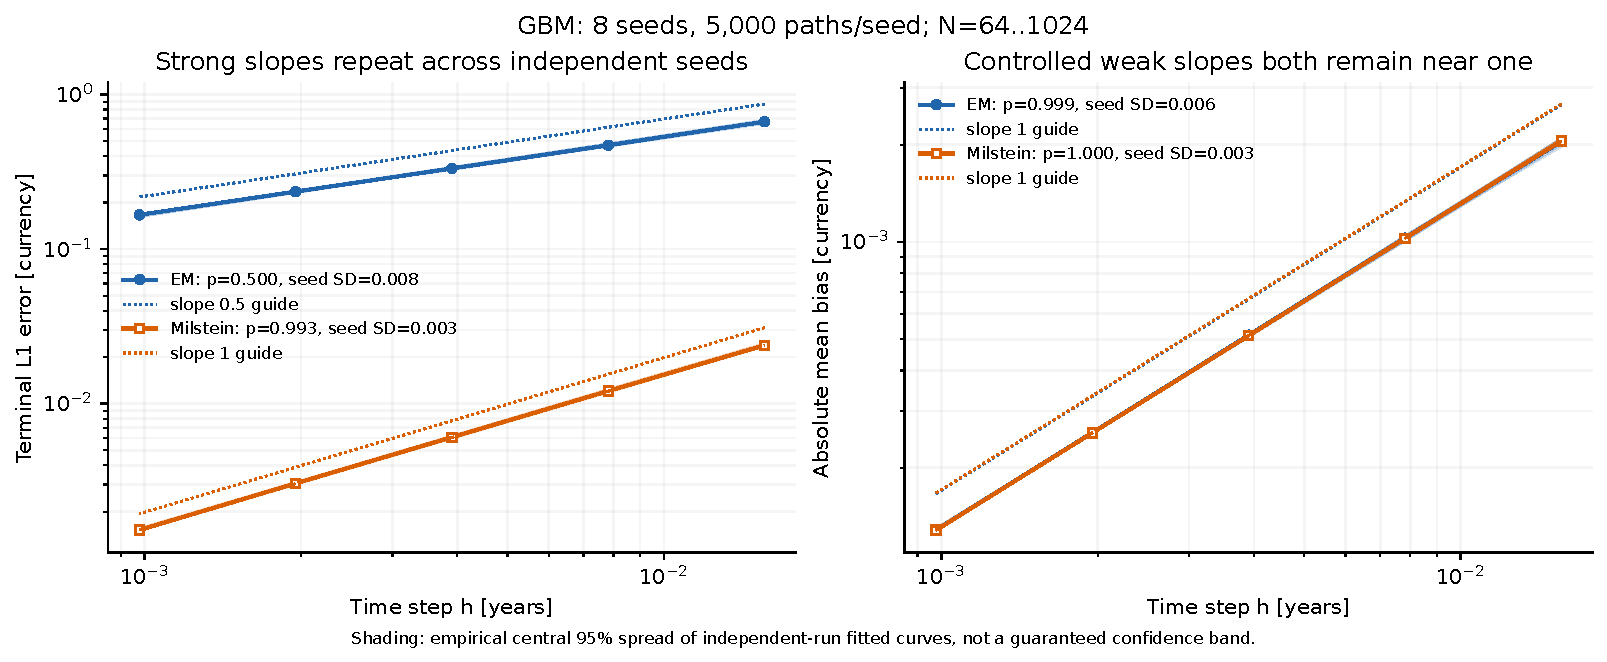
\includegraphics[width=.93\textwidth]{submission_gbm_repeat_slopes.pdf}
\caption{Independent-seed GBM fits with theoretical guides. Shading is the empirical central 95\% spread of fitted curves across runs, not an independent-level regression band or a guaranteed confidence band. Strong and weak rates remain distinct.}\label{fig:gbm-repeat}\end{figure}
\begin{figure}[H]\centering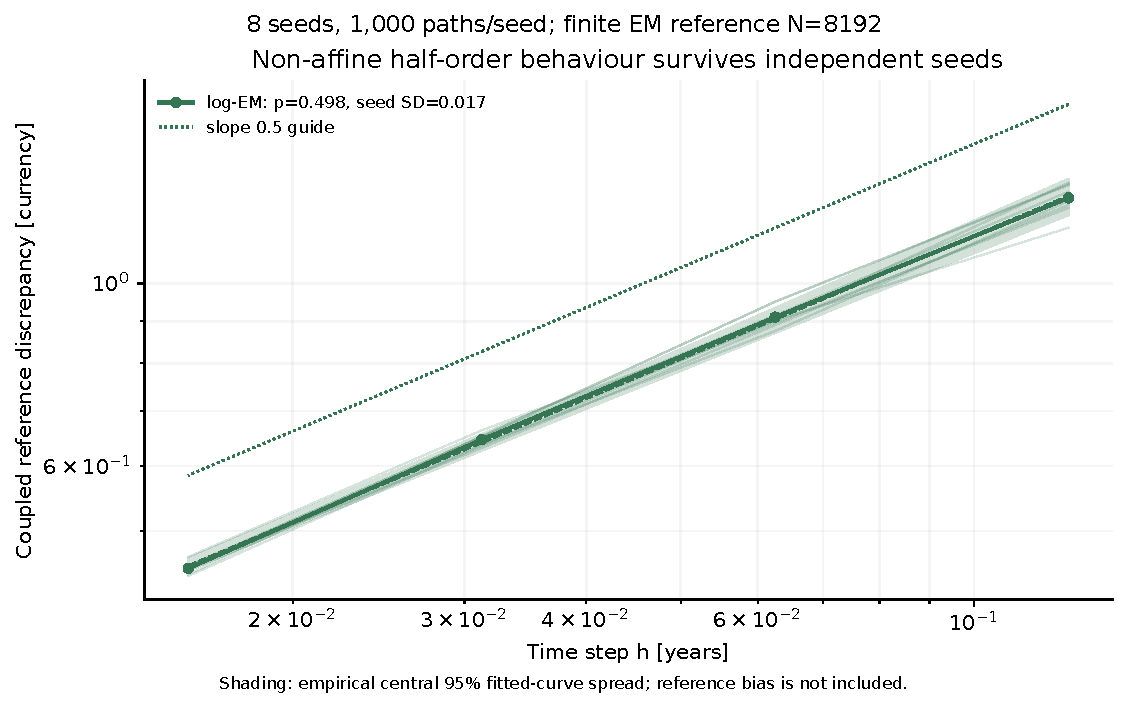
\includegraphics[width=.80\textwidth]{submission_nonaffine_repeat_slopes.pdf}
\caption{Non-affine strong fits vary across independent seeds but remain near half order for the same numerical reference. This spread does not include the unknown reference bias.}\label{fig:na-repeat}\end{figure}
Table~\ref{tab:repeat-rates} and Figures~\ref{fig:gbm-repeat}--\ref{fig:na-repeat} show the reproducibility of the fitted-rate conclusions. Only a small number of repeats is used; their empirical spread is descriptive. Coupled levels, finite fit windows and numerical references can produce systematic effects not included in a seed-only interval. In particular, Milstein's mean fitted strong slope is slightly below one and its sampling-only interval excludes one. This reflects a finite-window fitted quantity; it is not a confidence interval for the asymptotic theoretical order.

